\documentclass[a4paper, 14pt]{article}
\usepackage{tocloft}

\usepackage{amsthm}
\newtheorem{theorem}{Теорема}
\newtheorem{lemma}{Лемма}

\usepackage{setspace}
%\полуторный интервал
\onehalfspacing

\usepackage{arxiv}

\usepackage[T2A]{fontenc}
\usepackage[utf8]{inputenc}
\usepackage[english, russian]{babel}
% \usepackage{cmap}
\usepackage{url}
\usepackage{booktabs}
\usepackage{nicefrac}
\usepackage{microtype}
\usepackage{lipsum}
\usepackage{graphicx}
\usepackage{subfig}
\usepackage[square,sort,comma,numbers]{natbib}
\usepackage{doi}
\usepackage{multicol}
\usepackage{multirow}
\usepackage{tabularx}
\usepackage{color,colortbl} % Раскраска таблицы
\definecolor{Gray}{gray}{0.9}

\usepackage{tikz}
\usetikzlibrary{matrix}

% Algorithms
\usepackage{algpseudocode}
\usepackage{algorithm}

%% Шрифты
\usepackage{euscript} % Шрифт Евклид
\usepackage{mathrsfs} % Красивый матшрифт
\usepackage{extsizes} % Возможность сделать 14-й шрифт

\usepackage{makecell} % diaghead in a table
\usepackage{amsmath,amsfonts,amssymb,amsthm,mathtools,dsfont}
\usepackage{icomma}

\newcommand{\bz}{\mathbf{z}}
\newcommand{\bx}{\mathbf{x}}
\newcommand{\by}{\mathbf{y}}
\newcommand{\bv}{\mathbf{v}}
\newcommand{\bw}{\mathbf{w}}
\newcommand{\ba}{\mathbf{a}}
\newcommand{\bb}{\mathbf{b}}
\newcommand{\bp}{\mathbf{p}}
\newcommand{\bq}{\mathbf{q}}
\newcommand{\bt}{\mathbf{t}}
\newcommand{\bu}{\mathbf{u}}
\newcommand{\bs}{\mathbf{s}}
\newcommand{\bT}{\mathbf{T}}
\newcommand{\bX}{\mathbf{X}}
\newcommand{\bZ}{\mathbf{Z}}
\newcommand{\bS}{\mathbf{S}}
\newcommand{\bH}{\mathbf{H}}
\newcommand{\bW}{\mathbf{W}}
\newcommand{\bY}{\mathbf{Y}}
\newcommand{\bU}{\mathbf{U}}
\newcommand{\bQ}{\mathbf{Q}}
\newcommand{\bP}{\mathbf{P}}
\newcommand{\bA}{\mathbf{A}}
\newcommand{\bB}{\mathbf{B}}
\newcommand{\bC}{\mathbf{C}}
\newcommand{\bE}{\mathbf{E}}
\newcommand{\bF}{\mathbf{F}}
\newcommand{\bomega}{\boldsymbol{\omega}}
\newcommand{\btheta}{\boldsymbol{\theta}}
\newcommand{\bgamma}{\boldsymbol{\gamma}}
\newcommand{\bdelta}{\boldsymbol{\delta}}
\newcommand{\bPsi}{\boldsymbol{\Psi}}
\newcommand{\bpsi}{\boldsymbol{\psi}}
\newcommand{\bxi}{\boldsymbol{\xi}}
\newcommand{\bchi}{\boldsymbol{\chi}}
\newcommand{\bzeta}{\boldsymbol{\zeta}}
\newcommand{\blambda}{\boldsymbol{\lambda}}
\newcommand{\beps}{\boldsymbol{\varepsilon}}
\newcommand{\bZeta}{\boldsymbol{Z}}
% mathcal
\newcommand{\cX}{\mathcal{X}}
\newcommand{\cY}{\mathcal{Y}}
\newcommand{\cW}{\mathcal{W}}

\newcommand{\dH}{\mathds{H}}
\newcommand{\dR}{\mathds{R}}
% transpose
\newcommand{\T}{^{\mathsf{T}}}

% \renewcommand{\shorttitle}{\textit{arXiv} Шаблон}
\renewcommand{\epsilon}{\ensuremath{\varepsilon}}
\renewcommand{\phi}{\ensuremath{\varphi}}
\renewcommand{\kappa}{\ensuremath{\varkappa}}
\renewcommand{\le}{\ensuremath{\leqslant}}
\renewcommand{\leq}{\ensuremath{\leqslant}}
\renewcommand{\ge}{\ensuremath{\geqslant}}
\renewcommand{\geq}{\ensuremath{\geqslant}}
\renewcommand{\emptyset}{\varnothing}

\usepackage{hyperref}
% \usepackage[usenames,dvipsnames,svgnames,table,rgb]{xcolor}

\hypersetup{
	unicode=true,
	pdftitle={A template for the arxiv style},
	pdfsubject={q-bio.NC, q-bio.QM},
	pdfauthor={David S.~Hippocampus, Elias D.~Striatum},
	pdfkeywords={First keyword, Second keyword, More},
	colorlinks=true,
	linkcolor=black,        % внутренние ссылки
	citecolor=blue,         % на библиографию
	filecolor=magenta,      % на файлы
	urlcolor=blue           % на URL
}

\graphicspath{{../figures/}}

\usepackage{enumitem} % Для модификаций перечневых окружений

\theoremstyle{definition} % "Определение"
\newtheorem{definition}{Опр.}[section]

\usepackage{etoolbox}

\makeatletter
\expandafter\patchcmd\csname\string\algorithmic\endcsname{\itemsep\z@}{\itemsep=1.5mm}{}{}
\makeatother
%%% Титульный лист
% \input{title}
% \setcounter{page}{2}

\renewcommand{\abstractname}{Аннотация}

\title{Методы векторного представления глубоких генеративных моделей}

\author{
    Мария Никитина \\
    \texttt{nikitina.mariia@phystech.edu} \\
    \And
    Антон Бишук \\
    \texttt{anton.bishuk@mail.ru} \\
    \And
    Олег Бахтеев \\
    \texttt{bakhteev(at)phystech.edu}
}
\date{\today}

\usepackage{setspace}
%\полуторный интервал
\onehalfspacing

\begin{document}
\maketitle
% \input{title}
\setcounter{page}{2}

\begin{abstract}
Увеличение времени и ресурсов, затрачиваемых на обучение больших моделей привели к появлению большого количества работ, направленных на поиск уже существующей обученной модели, подходящей под новую задачу. Множество исследований направлено на поиск пространства моделей-датасетов, с помощью которого можно отыскать уже существующую модель, хорошо подходящую под новую задачу. Однако, исследования проводятся в основном в области дискриминативных моделей. Эта работа направлена на поиск векторного представления генеративных моделей, описывающего статистические свойства датасетов, на которых они обучены. Таким образом с помощью такого пространства можно подбирать подходящую генеративную модель, используя привычные операции с векторами. Эксперименты проводятся на VAE и Autoencoder.
\end{abstract}

% \keywords{Генеративные модели \and Векторное представление \and Статистические свойства моделей}

\newpage
% \pagenumbering{roman} % use lowercase Roman numerals for page numbering before the main content

% \tableofcontents
% \clearpage % start the table of contents on a new page

% \pagenumbering{arabic}

\section{Введение}
Пусть задан некоторый набор генеративных моделей, описывающий разные выборки/генеральные совокупности данных. Требуется предложить метод векторного представления этих моделей, который будет сохранять статистические свойства данных. С помощью такого представления можно облегчить поиск подходящей обученной модели  без больших затрат времени и ресурсов на обучения. Также поиск по пространству генеративных моделей может быть применим для анализа качества работы разных архитектур на задаче генерации требуемых данных.

Векторное пространство должно отвечать следующим требованиям:

\begin{enumerate}
    \item Расстояние между векторными представлениями моделей для близких выборок должно быть невелико (при условии, что сами модели хорошо их описывают);

    \item Модели, обученные на композиции/смеси выборок должны учитывать свойства всех выборок, входящих в смесь.
\end{enumerate}

Для выполнения данных требования и решения задачи в данной статье исследуются и сравниваются три варианта решения:

\begin{enumerate}
    \item Один из возможных вариантов: сумма векторных представлений моделей, полученных по датасетам $D_1$, $D_2$ должна приблизительно соответствовать векторному представлению датасета $D_1 + D_2$. Пример для итогового пространства в виде единичной сферы представлен на рис. \ref{fg:classes};
    
    \item Вместо использования евклидового расстояния на векторных представлениях, использовать иерархию;
    
    \item Представить модель как граф и работать с пространством графов.
\end{enumerate}

\begin{figure}
    \begin{center}
    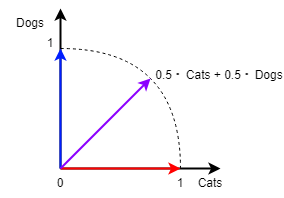
\includegraphics[width=0.7\linewidth]{Presentation/Pictures/Classes.png}
    \caption{Требуемое соотношение между моделями в векторном пространстве}
    \label{fg:classes}
    \end{center}
\end{figure}

\section{Вычислительные эксперименты}
\subsection{Архитектура}

\begin{figure}{}
    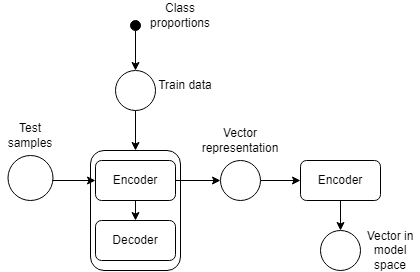
\includegraphics[width=1.0\linewidth]{Presentation/Pictures/Model.png}
    \caption{Архитектура эксперимента}
    \label{fg:model}
\end{figure}

Архитектура решения представлена на рис \ref{fg:model}.

\begin{enumerate}
    \item Случайное сэмплирование долей классов в датасете для $n$ моделей;

    \item Обучение $n$ моделей на соответствующих датасетах;

    \item Получение векторов из обученных моделей;

    \item Обучение энкодера на полученных моделях. Предсказание:
        \begin{enumerate}
            \item Вектора на части единичной сферы

            \item Расстояния между двумя моделями
        \end{enumerate}
\end{enumerate}

Метрики для реализации обучения:

\begin{enumerate}
    \item Contrastive N-pair loss, где $\text{Encoder}(m_i) = \textbf{x}$, $\textbf{d}_i = \textbf{x}_i^+$, остальные элементы батча: $\textbf{x}_i^-$:

\[\mathcal{L}_{N-pair}(f) = - \log \frac{\exp(\textbf{x}^T \textbf{x}_i^+)}{\exp(\textbf{x}^T \textbf{x}_i^+) + \sum _{i=1}^{N-1} \exp(\textbf{x}^T\textbf{x}_i^-)};\]
    \item Угол между вектором модели $\text{Encoder}(m_i)$ и датасета $\textbf{d}_i$:

\[\mathcal{L}_{cos}(\text{Encoder}(m_i), \textbf{d}_i) = \cos(\text{Encoder}(m_i) \cdot \textbf{d}_i);\]

    \item Triplet loss:

\[\mathcal{L}_{Triplet} = \sum\limits_{x \in \chi}\max(0, ||\textbf{x} - \textbf{x}^+||_2^2 - ||\textbf{x} - \textbf{x}^-||_2^2 + \epsilon;\]

    \item MSE между $\text{Encoder}(m_i)$ и $\textbf{d}_i$:

\[\mathcal{L}_{MSE}(\text{Encoder}(m_i), \textbf{d}_i) = \|\text{Encoder}(m_i) - \textbf{d}_i)\|_2^2.\]
\end{enumerate}

\subsection{Предсказание вектора в пространстве моделей-датасетов}

Для базового эксперимента берётся 3 наиболее удалённых класса из датасета CIFAR. Для поиска таких классов использовалось евклидово расстояние на ембеддингах, полученных из выходного слоя ResNet.
\end{document}